\documentclass[11pt, oneside]{scrartcl}   	% use "amsart" instead of "article" for AMSLaTeX format

%%%%%%%%%%%%%%%%%%%%%%%%%%%%%%%%%%%%%%%%%%%%%%%%%%%%%%%%%%%%%%%%%%%%%%%
% packages
\usepackage[portrait]{geometry}               		% See geometry.pdf to learn the layout options. There are lots.
\geometry{a4paper}                   		% ... or a4paper or a5paper or ...
%\geometry{landscape}                		% Activate for rotated page geometry
%\usepackage[parfill]{parskip}    		% Activate to begin paragraphs with an empty line rather than an indent
\usepackage{graphicx}				% Use pdf, png, jpg, or eps with pdflatex; use eps in DVI mode
							% TeX will automatically convert eps --> pdf in pdflatex
\usepackage{amssymb}
\usepackage{amsmath}
\usepackage{tikz}
\usepackage{tikz-3dplot}
\usepackage{mathtools}
\usepackage{pgfplots}
\usetikzlibrary{angles, quotes}
\pgfplotsset{width=7cm,compat=newest}
\usepackage{listings}
\usepackage[d]{esvect}
\usepackage{color}
\usepackage{eso-pic}
\usepackage{hyperref}


% \include{mydefines}

%%%%%%%%%%%%%%%%%%%%%%%%%%%%%%%%%%%%%%%%%%%%%%%%%%%%%%%%%%%%%%%%%%%%%%%
% color definitions
\definecolor{mygreen}{rgb}{0,0.6,0}
\definecolor{mygray}{rgb}{0.5,0.5,0.5}
\definecolor{mymauve}{rgb}{0.58,0,0.82}


%%%%%%%%%%%%%%%%%%%%%%%%%%%%%%%%%%%%%%%%%%%%%%%%%%%%%%%%%%%%%%%%%%%%%%%
% definitions for listings
\lstset{ 
	backgroundcolor=\color{white},   % choose the background color; you must add \usepackage{color} or \usepackage{xcolor}; should come as last argument
	basicstyle=\footnotesize,        % the size of the fonts that are used for the code
	breakatwhitespace=false,         % sets if automatic breaks should only happen at whitespace
	breaklines=true,                 % sets automatic line breaking
	captionpos=b,                    % sets the caption-position to bottom
	commentstyle=\color{mygreen},    % comment style
	deletekeywords={...},            % if you want to delete keywords from the given language
	escapeinside={\%*}{*)},          % if you want to add LaTeX within your code
	extendedchars=true,              % lets you use non-ASCII characters; for 8-bits encodings only, does not work with UTF-8
	firstnumber=1000,                % start line enumeration with line 1000
	frame=single,	                   % adds a frame around the code
	keepspaces=true,                 % keeps spaces in text, useful for keeping indentation of code (possibly needs columns=flexible)
	keywordstyle=\color{blue},       % keyword style
	language=Octave,                 % the language of the code
	morekeywords={*,...},            % if you want to add more keywords to the set
	numbers=left,                    % where to put the line-numbers; possible values are (none, left, right)
	numbersep=5pt,                   % how far the line-numbers are from the code
	numberstyle=\tiny\color{mygray}, % the style that is used for the line-numbers
	rulecolor=\color{black},         % if not set, the frame-color may be changed on line-breaks within not-black text (e.g. comments (green here))
	showspaces=false,                % show spaces everywhere adding particular underscores; it overrides 'showstringspaces'
	showstringspaces=false,          % underline spaces within strings only
	showtabs=false,                  % show tabs within strings adding particular underscores
	stepnumber=2,                    % the step between two line-numbers. If it's 1, each line will be numbered
	stringstyle=\color{mymauve},     % string literal style
	tabsize=2,	                   % sets default tabsize to 2 spaces
	title=\lstname                   % show the filename of files included with \lstinputlisting; also try caption instead of title
}

%%%%%%%%%%%%%%%%%%%%%%%%%%%%%%%%%%%%%%%%%%%%%%%%%%%%%%%%%%%%%%%%%%%%%%%
% headlines and footlines
\usepackage[headsepline]{scrlayer-scrpage}
\pagestyle{scrheadings}
\clearpairofpagestyles
% \ohead{\textsf{Section \thesection}}  % \thesection
\ohead{\headmark}
\automark[subsection]{section}

% \chead{\textsf{Page \thepage}}
\chead[\pagemark]{Page \pagemark}
\ihead{\textsf{Project Description}}
\cfoot[\pagemark]{Page \pagemark}
%%%%%%%%%%%%%%%%%%%%%%%%%%%%%%%%%%%%%%%%%%%%%%%%%%%%%%%%%%%%%%%%%%%%%%%

\setlength{\parindent}{0pt}

%%%%%%%%%%%%%%%%%%%%%%%%%%%%%%%%%%%%%%%%%%%%%%%%%%%%%%%%%%%%%%%%%%%%%%%
% new commands
\newcommand{\mb}[1]{{\mathbf #1}}

\begin{document}

%%%%%%%%%%%%%%%%%%%%%%%%%%%%%%%%%%%%%%%%%%%%%%%%%%%%%%%%%%%%%%%
% title page
\begingroup
	\thispagestyle{empty}
	\centering
	\AddToShipoutPicture*{\put(30,100){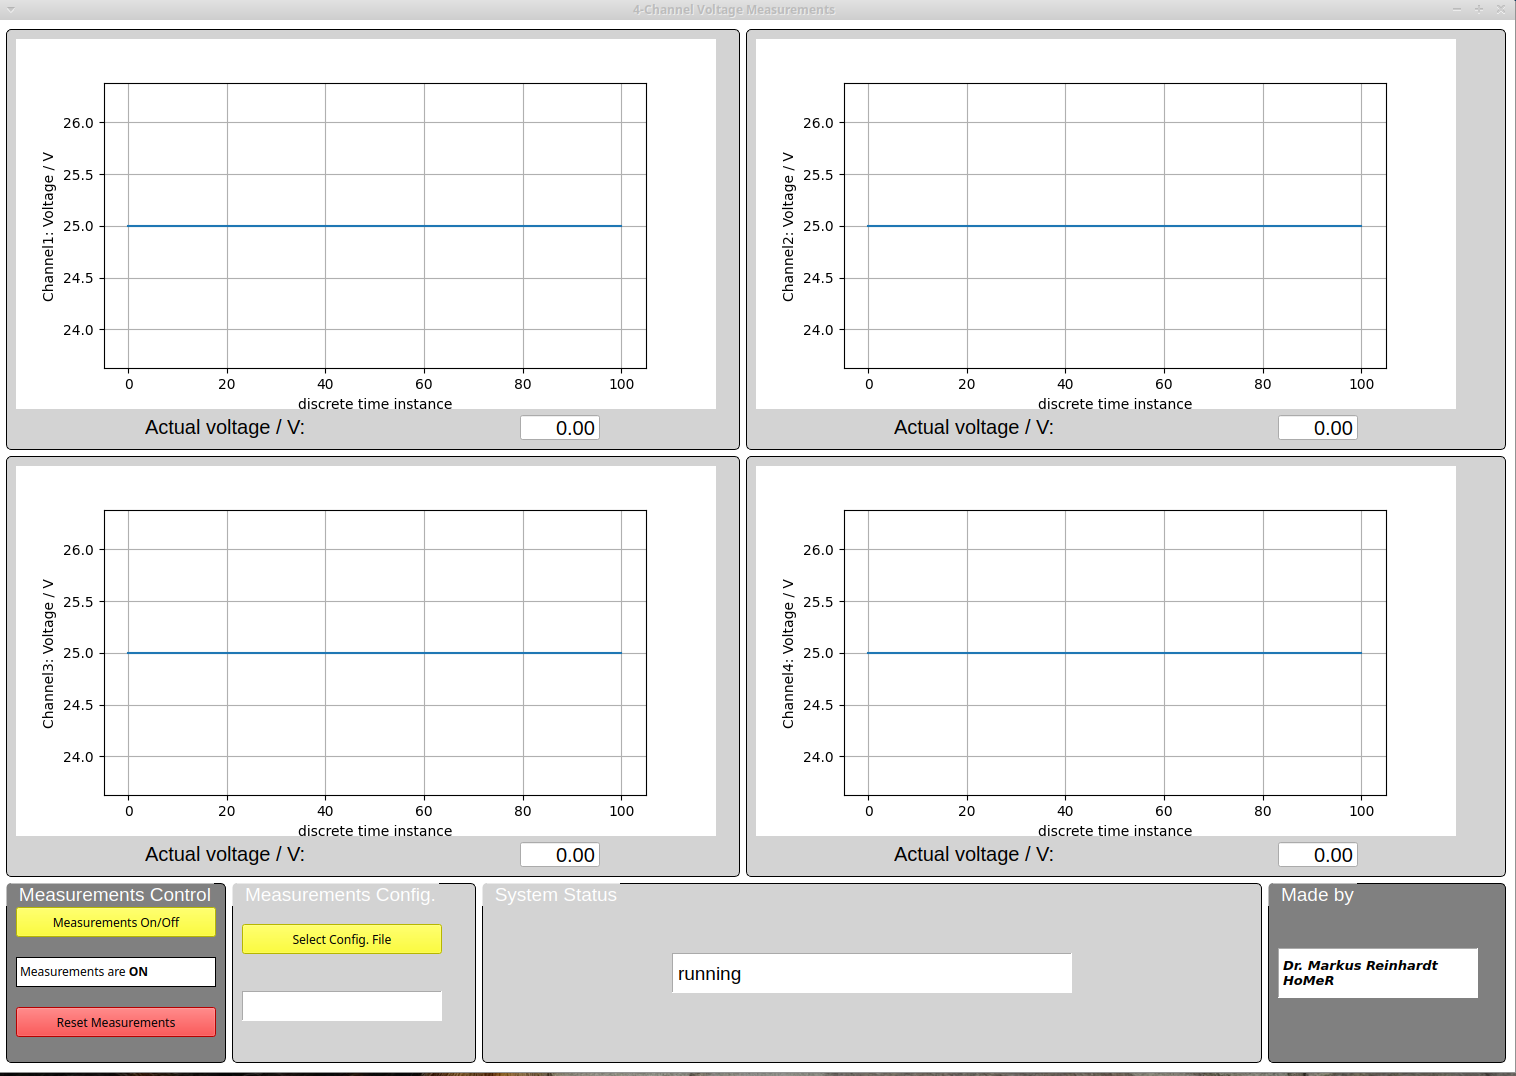
\includegraphics[scale=0.35]{Figures/ApplicationWindow.png}}} % Image background
	\par\normalfont\fontsize{30}{30}\sffamily\selectfont
	\vspace*{1.0cm}
	{\color{blue}
		\textbf{\Huge My Simple 4-Channel DAS} \\ 
		\textbf{\huge Description and Evaluation} \\
		\vspace*{0.5cm}
		\hspace{-0.3cm}
		{\textbf\huge by Dr. Markus Reinhardt }\par % Book title
		\hspace{-1.3cm}
		{\textbf \huge  \today}\par % Author name
		\vspace*{1.5cm}
	}
\endgroup
\vfill

%%%%%%%%%%%%%%%%%%%%%%%%%%%%%%%%%%%%%%%%%%%%%%%%%%%%%%%%%%%%%%%
% table of contents
\newpage
\thispagestyle{empty}
\tableofcontents
\newpage

%%%%%%%%%%%%%%%%%%%%%%%%%%%%%%%%%%%%%%%%%%%%%%%%%%%%%%%%%%%%%%%
% lists of figures and tables
\newpage
\thispagestyle{empty}
\listoffigures
\listoftables

%%%%%%%%%%%%%%%%%%%%%%%%%%%%%%%%%%%%%%%%%%%%%%%%%%%%%%%%%%%%%%%
% the main text
\newpage
\pagestyle{scrheadings}
\section{Concept description}
A project to build-up a simple 4-channel low sample rate, high accuracy (16-bit ADC)
Data Acquisition System (DAS) to support general universal measurements.\\

The signals to be measured are fed to a 1:10 divider or via a 1:1 connection to the buffer amplifier of each channel.
The signals are then ADC converted by the 4 channel ADS1115 ADC on the ADC module.
The Arduino Uno is controlling the ADS1115 and receiving the digitized signals via the I2C interface.
The data is then sent to the PC via the SoftwareSerial port, a USB/Serial module using the CmdMessenger library to the PC.
On the PC a Python (PyQt) or C++ (Qt) program using also the (Py)CmdMessenger library is receiving, evaluating and displaying the data.

HW components:
\begin{itemize}
	\item Arduino Uno
	\item USB/Serial module to connect the PC with the Uno via SoftwareSerial interface and USB connector.
	\item 4-Channel ADS1115 16-bit ADC module.
	\item 4-Channel 1x buffer amplifier board, LM324 based.
	\item 10x / 1x inputs and resistor divider.
	\item Simple plastic case
\end{itemize}

SW components:
\begin{itemize}
	\item Arduino sketch to control the ADC module and send the data via the serial interface to the PC.
	\item C++ / Qt based software library to sample, store and evaluate data from up to 4 channels.
	\item PyQt based Python program running on the PC to receive and store data from up to 4 channels.
	\item First SW example: Tracing the charging characteristic (voltage and current) of a LiPo cell.
\end{itemize}

\section{Hardware setup}
The used ADC module is shown in figure \ref{fig:HWSetup}.
\begin{figure}[htbp]
	\centering
	\label{fig:HWSetup}
	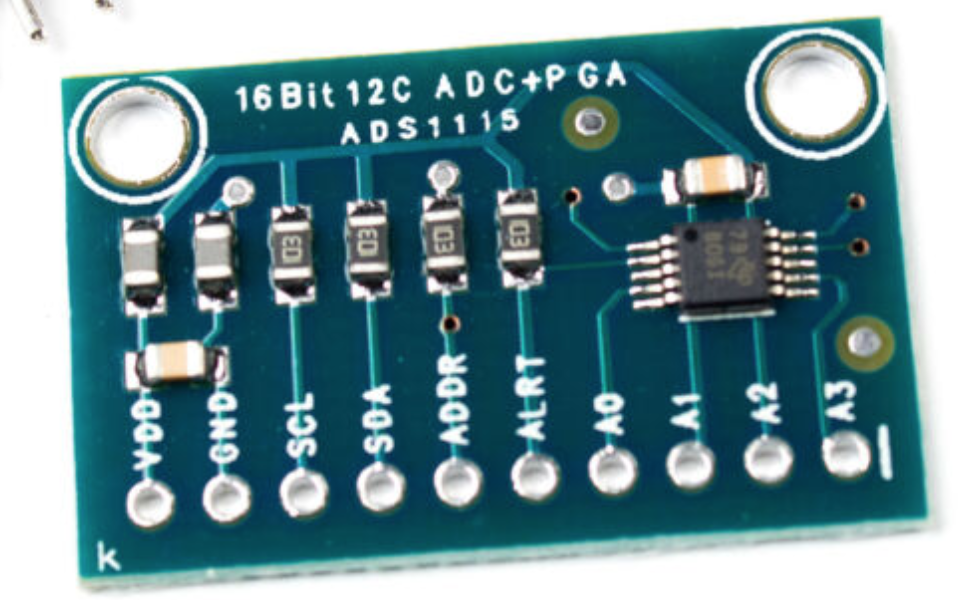
\includegraphics[width=1.0\linewidth]{Figures/ADS1115ADCBoard.png}
	\caption{ADC module with ADS1115}
\end{figure}

\newpage
\section{Schematics}
The schematics are shown in figure \ref{fig:Schematics}.
\begin{figure}[htbp]
	\centering
	\label{fig:Schematics}
	\includegraphics[width=1.0\linewidth]{Figures/MySimple4ChannelDAS.pdf}
	\caption[Schematics]{Schematics}
\end{figure}

\newpage
\section{Software setup}
\subsection{PC Application}
The GUI of the PC application is shown in figure \ref{fig:ApplicationWindow}.
\begin{figure}[htbp]
	\centering
	\label{fig:ApplicationWindow}
	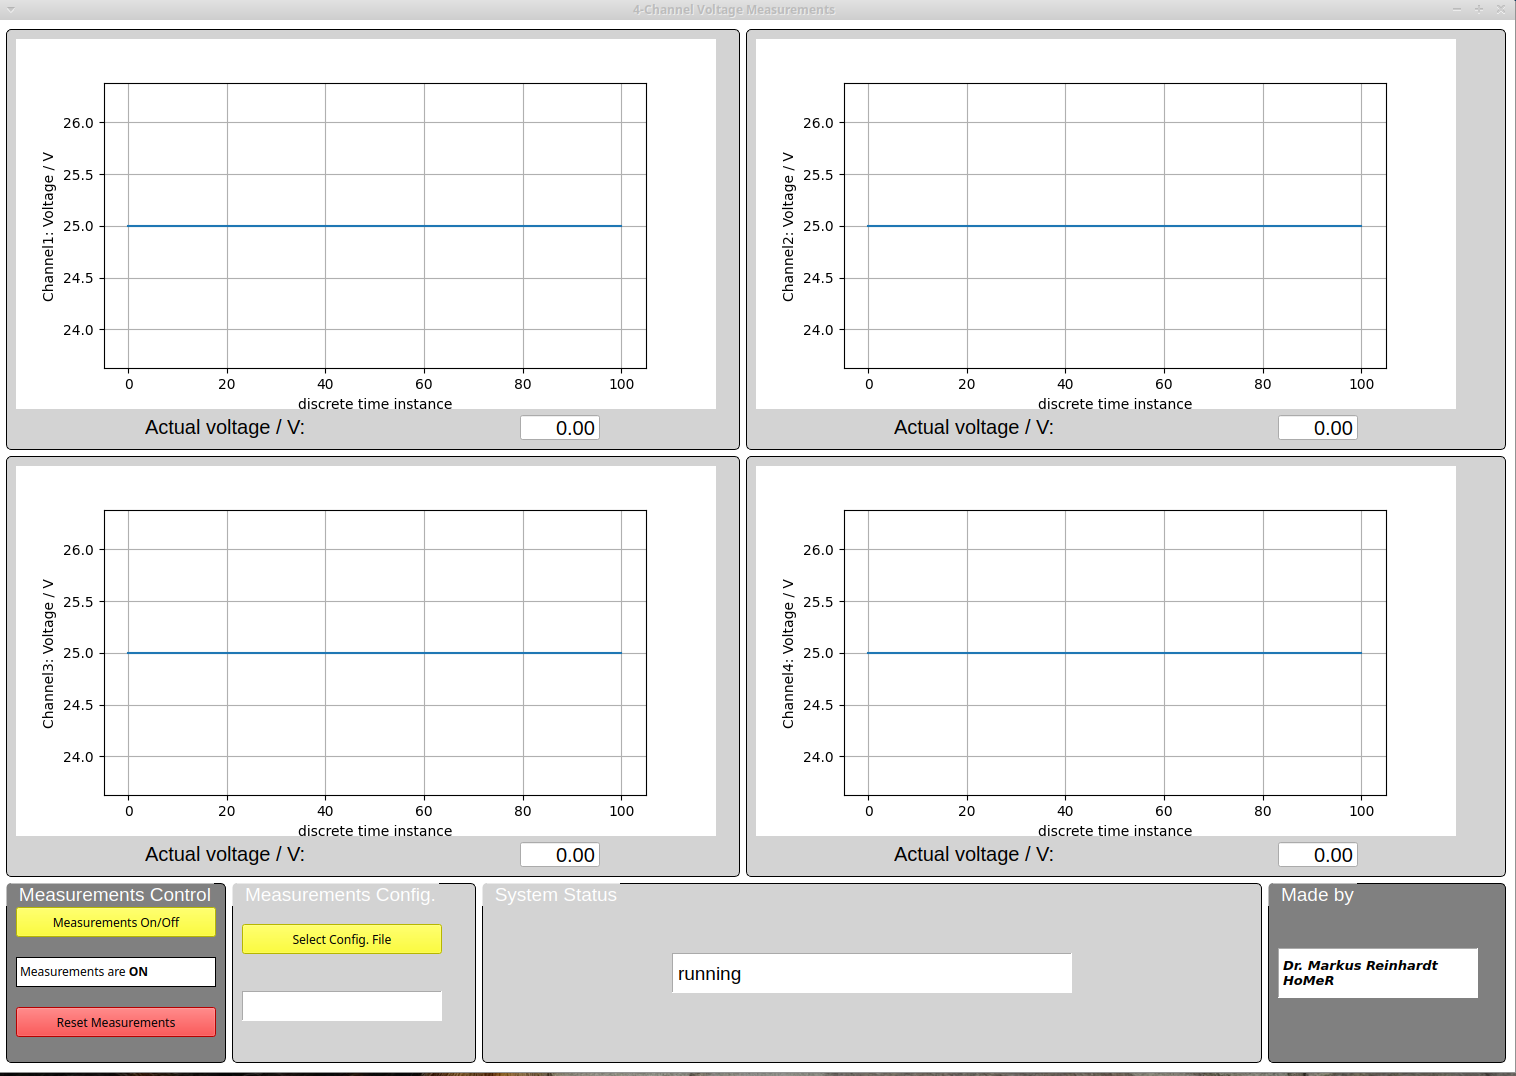
\includegraphics[width=1.0\linewidth]{Figures/ApplicationWindow.png}
	\caption[PC Application]{PC Application}
\end{figure}
\newpage

\appendix
\section{Appendix A}
\subsection{Appendix A.1}	

\end{document}